\documentclass[12pt, twosides]{book}
\usepackage{amsmath}
\usepackage{graphicx}
\usepackage{color}
\begin{document}

\chapter{Chapter 2}
\section{Dark Matter ALPs}

There is strong astrophysical evidence that a large portion of the matter in our galaxy is non-luminous, meaning that it does not have electromagnetic interactions. The first evidence came from measurements by Oort \cite{oort32}, who showed that their must be more mass in the Milky Way than measured; at around the same time, Fritz Zwicky \cite{zwicky37} measured the mass to light ratio in the Coma cluster. He found that the MtoL ratio was nearly 500 times greater than that expected. Most definitively, measurements of spiral galaxies using hydrogen's hyperfine transition at 21 cm have shown that in a a survey of many glaxies, all of them have rotation curves that suggest that the matter is distributed in a diffuse halo, not concentrated near the center, as the light is\cite{rubin80}. This dark matter would affect structure formation; as pockets of local overdensity formed, non-relativistic dark matter would settle into the gravitational well and provide many sites of small structure, which could then accrete to form large structure later - this is consistent with the level of temperature anisotropies observed in the Cosmic Microwave background \cite{planck13}, and n-body simulations [NEEDSREF]. Observations of temperature anisotropies in the Cosmic Microwave Background also allow us to make predictions on cosomological parameters; $\kappa$, the geometry of the universe, and $\Omega$, the matter density. The measurement of the relative amplitude of the anisotropies tells us that the baryon density of the universe is 4%. This rules out the simplest assumption that dark matter is baryonic and made of dead stars or non-luminous brown dwarfs. This was also ruled out by micro-lensing surveys of Massic Compact Halo Objects (MACHOS) [NEEDSREF], which did not find as many events as would be predicted by the abundance of dark matter. The measurements of supernova with respect to distance, using them as standard candles, tells us how much of the universe is made up on dark energy, a mysterious substance which is causing the expansion of the universe to accelerate. The amount of dark energy in the universe, taken from CMB measurements, is 73%. The remaining 21% is dark matter.

The lambda cold dark matter model ($\Lambda$ CDM) supposes non-relativistic, non-baryonic particulate dark matter. 

There are three strong candidates for the particle of dark matter: sterile neutrinos, WIMPs and axions. Sterile Neutrinos are neutrinos which are right handed, and thus do not interact with the electroweak force, which only deals with left-handed neutrinos. There is some evidence for a 3.5 keV line in some galaxies which would correspond to a 7 keV sterile neutrino [NEEDSREF].

Weakly Interacting Massive Particles (WIMPs) are stable neutral particles with large mass, usually in the tens of GeV to some TeV range. These particles would have the correct dark matter density if their cross section for interactions is equal to the electroweak scale, a suggestive coincidence called the "WIMP miracle". There are also supersymmetric theories extending the Standard Model; these SUSY theories predict a super partner for every elementary particle with opposite spin, ie. every fermion has a boson partner and vice versa. SUSY theories are important for solving a problem in particle physics, which is that the Higgs mass is divergent when including higher order corrections. The lightesst SUSY partner, the neutralino, has the correct properties to be cold dark matter (spinless, chargeless) and would constitute a WIMP. There are direct and indirect searches looking for WIMPs, either through their rare scattering off of a nuclei such as LUX \cite{lux14}, or through indirect searches which assume that WIMPS are their own antiparticle and then annihilate, producing visible signatures in the galaxy [NEEDSREF]. There is some evidence from the Fermi gamma ray telescope for a WIMP like signal coming from the center of the galaxy [NEEDSREF].

Lastly, the axion is also a strongly motivated cold dark matter candidate. The axion, as described below, arises from the symmetry breaking of a symmetry introduced to solve the strong CP problem by dynamically tending the P and T violating term in QCD to zero. The axion, due to astrophysical and laboratory constraints, would need to be less than approximately 1 meV; in the models of the axion, it's coupling is related to the mass, so these light axions have extremely feeble couplings to matter, making them good dark matter candidates. They can be produced thermally, making them hot dark matter candidates, or non-thermally, either through the vacuum misalignment mechanism [NEEDSREF], through cosmic strings [NEEDSREF], or topological defects [NEEDSREF].

The argument for non-relativistic matter today usually relies on thermalization arguments; which imply that the heavier the matter, the cooler, or more non-relativistic it is today. However, there are other mechanisms by which very light particles could be produced in the early universe such that they are non-relativistic today.

\subsection{$U(1)_{PQ}$ symmetry}

To describe this mechanism we first have to describe the mechanism of symmetry breaking which gives rise to light particles. To do so, we will go through the process which gives rise to the canonical axion. This process was postulated by Peccei and Quinn in 1977 \cite{peccei77} as a natural way to produce CP conservation the theory of strong interactions, Quantum Chromodynamics. 

The Peccei-Quinn solution to this strong CP problem, as it is known, was to introduce a global chiral U(1) symmetry, denoted $U(1)_{PQ}$. This symmetry can be spontaneously broken at some energy scale $f_a$, producing massless Goldstone bosons from the azimuthal degree of freedom (this is the axion), and some high energy mode from the radial degree of freedom; this was deemed to be the two Higgs doublets in the original theory, which sets the energy scale.  There are many models that construct other scalars as the radial mode, allowing the energy scale to decouple from the electroweak scale \cite{kim79} \cite{shifman80}, \cite{dine81}, \cite{zhitnitsky80}.

The axion acquires mass through explicit symmetry breaking of the$U(1)_{PQ}$ symmetry with QCD. This occurs because of a chiral anomaly \cite{jackiw76}. In all respects this is analogous to the process by which the pion, the Goldstone boson of the axial $U(1)_A$, acquires its mass through a chiral anomaly. The mass that the axion acuqires is proportional to $m_a \sim \Lambda_{QCD}^2/f_a$. The axion coupling to matter is inversely proportional to the energy scale $f_a$ and thus proportional to the mass.

Using Higgs doublets would give one a rough prediction for the axion mass of 150 keV; this axion would have a lifetime of 1 microsecond and would have been detected in collider experiments through quarkonium decays and beam dump experiments \cite{crystalball90}. The branching ratios observed were significantly less than predicted; thus this axion was ruled out.

However, as stated above, the symmetry can come from other scalars; which would separate $f_a$ from the electroweak scale and let it be much higher, and so the axion coupling and mass would be much weaker. In 1983 Pierre Sikivie proposed using the axion to two photon coupling \cite{sikivie83} to search for axions, and proposed that axions would make good dark matter candidates. This interaction is the Primakoff effect, which can be written effectively as $E \dot B$. With strong magnetic fields, the axion to two photon transition is made much stronger.

Note, I say axion here, but these searches apply for axion-like particles in general. The only difference is that axion-like particles do not have the relationship between coupling and mass, so there are two free parameters in the theory.

In order for ALPs to be good dark matter candidates, they must have the correct abundance. We now go over how ALPs could be produced in the early universe such as to have the correct density today.

\subsection{Misalignment Mechanism}

We have covered how, by the addition of a global symmetry that has explicit symmetry breaking at some high energy scale, a low mass boson can arise. The mass of this particle will "turn on" when the energy scale at which the symmetry breaking occurs is matched in the energy scale of the universe (or more commonly described, the temperature). If we think of the initial 2$\pi$ degrees of freedom of the azimuthal mode, a simple picture would be of the tipping of the $\phi^4$ potential, or the wine bottle potential, leading to the angle to settle at one particular value. As the angle $\theta$ must approach its minimum, there will be oscillations around that point. These oscillations will be affected by the expansion of the universe; one can write a damped harmonic oscilllator equation of motion [NEEDSREF] where H is the hubble parameter.

\begin{align*}
\ddot \bar{\theta} + 3H(t)\dot \bar{\theta} + m_a^2\sin(\bar{\theta}) = 0
\end{align*}

As long as $\theta$ is not too small, these damped oscillations will result in a present day energy density roughly equal to the dark matter density we observe [NEEDSREF].

\begin{figure}
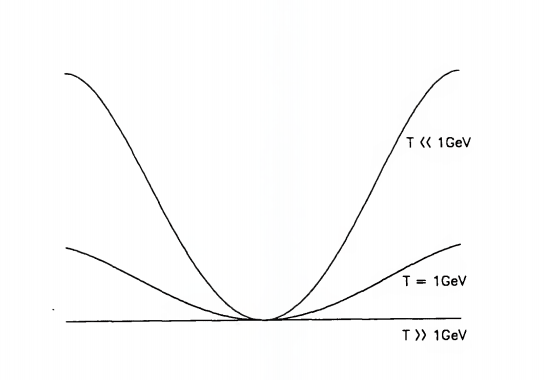
\includegraphics[width=0.7\textwidth]{differentpotentials}
\end{figure}

The cosmological history is also affected by whether the mass is turned on before or after inflation. With the 2014 BICEP result [NEEDSREF], we can set the scale of inflation at $10^{14} GeV$. If the axion acquires mass before inflation, then there is a uniform axion mass in our horizon; otherwise, there might be several causal patches with axion masses at different values, and we can only average over them to get a predicted value [NEEDSREF].

\bibliographystyle{plain}
\bibliography{thesisbib}
\end{document}